\documentclass[UTF8,a4paper]{article}
\usepackage[UTF8]{ctex}
\usepackage{tikz}
\usepackage{geometry}
\usepackage{xcolor}
\usepackage{array}
\usepackage{fancyhdr}
\usepackage{colortbl}
\usepackage{longtable}

% 页面设置
\geometry{a4paper, left=2cm, right=2cm, top=2.5cm, bottom=2.5cm}

% 深蓝色主题颜色定义
\definecolor{deepblue}{RGB}{0,51,102}
\definecolor{lightblue}{RGB}{102,178,255}
\definecolor{safegreen}{RGB}{76,175,80}
\definecolor{warningyellow}{RGB}{255,193,7}
\definecolor{lilac}{RGB}{200,150,255}
\definecolor{warningorange}{RGB}{255,152,0}
\definecolor{riskred}{RGB}{220,38,127}

% 页眉页脚设置
\pagestyle{fancy}
\fancyhf{}
\renewcommand{\headrulewidth}{0pt}
\fancyfoot[C]{\small\color{gray}睿文智评AI预审评估系统 - AIGC检测报告}
\fancyfoot[L]{}
\fancyfoot[R]{}

% 禁止首页页码
\thispagestyle{empty}

\begin{document}
\setlength{\parindent}{0pt}

% ========== 封面页 ==========

% 深蓝色标题栏
{\color{deepblue}\hrule height 3pt}
\vspace{0.5cm}

\begin{center}
    {\Huge\bfseries\color{deepblue} AIGC检测结构化报告}\par
    \vspace{0.3cm}
    {\Large\color{gray} 睿文智评AI预审评估系统}
\end{center}

\vspace{0.8cm}

% 元数据表格和环图并排显示
\begin{center}
\begin{minipage}{0.55\textwidth}
% 左侧：元数据表格
\renewcommand{\arraystretch}{0.6}
\begin{tabular}{|p{2.5cm}|p{6cm}|}
\hline
\rowcolor{deepblue}
\color{white}\textbf{项目} & \color{white}\textbf{内容} \\
\hline
论文标题 & 基于矩阵略图的对数几率老虎机计算加速 \\
\hline
学生姓名 & 何临哲 \\
\hline
学号 & 211300034 \\
\hline
检测日期 & 2026年03月31日 \\
\hline
\end{tabular}
\end{minipage}%
\hfill
\begin{minipage}{0.35\textwidth}
% 右侧：环图和统计数据
\centering

\begin{tikzpicture}
  % 定义角度
  \def\aigcangle{116.09545620810991}

  % AIGC部分
  \draw[fill=safegreen,draw=none] (0,0) -- (0:1.6) arc (0:\aigcangle:1.6) -- (0,0);

  % 人工部分
  \draw[fill=lightblue,draw=none] (0,0) -- (\aigcangle:1.6) arc (\aigcangle:360:1.6) -- (0,0);

  % 内圆（环图效果）
  \draw[fill=white,draw=none] (0,0) circle (1.0);

  % 中心文本
  \node at (0,0) {
    \begin{tabular}{c}
    \Large\textbf{32.2\%} \\
    \small AIGC率
    \end{tabular}
  };

  % 图例
  \node[anchor=west,font=\small] at (-1.8,-1.2) {
    \begin{tabular}{@{}cl@{}}
    \textbf{AIGC} & 32.2\% \\
    \textbf{人工} & 67.8\%
    \end{tabular}
  };
\end{tikzpicture}

\vspace{0.1cm}
\begin{tabular}{ll}
\footnotesize
\textbf{总字数：} & 23439 \\
\textbf{疑似字数：} & 7558 \\
\textbf{人工写作字数：} & 15881 \\
\textbf{总体AIGC率：} & 32.2% \\
\end{tabular}
\end{minipage}
\end{center}

\vspace{0.3cm}

% 风险等级评估
\begin{center}
\renewcommand{\arraystretch}{1.2}
\begin{tabular}{|p{14cm}|}
\hline
\rowcolor{deepblue}
\color{white}\textbf{风险评估} \\
\hline
\textbf{风险等级：} \textbf{低} \\
\hline
\textbf{评估说明：} 论文整体AIGC含量较低，以人工创作为主。 \\
\hline
\end{tabular}
\end{center}

\newpage

% ========== 章节详细分析 ==========

\thispagestyle{fancy}

\begin{center}
{\Large\bfseries\color{deepblue} 章节详细分析}
\end{center}

\vspace{0.5cm}

% 章节分析表格
\begin{center}
\renewcommand{\arraystretch}{1.2}
\small  % 使用小字体
\begin{longtable}{|p{4.5cm}|p{1.3cm}|p{1.3cm}|p{4.5cm}|p{1.4cm}|}
\hline
\rowcolor{deepblue}
\color{white}\textbf{章节名称} &
\color{white}\textbf{总字数} &
\color{white}\textbf{疑似字数} &
\color{white}\textbf{AIGC占比} &
\color{white}\textbf{风险等级} \\
\hline

第一章 引言 &
1,790 &
1,251 &


\begin{tikzpicture}
  % 背景条
  \draw[fill=gray!20,draw=none] (0,0) rectangle (2.8,0.3);
  % 进度条
  \draw[fill=warningorange,draw=none] (0,0) rectangle (1.9581663164021816,0.3);
  % 百分比文本
  \node[right,font=\footnotesize] at (2.9,0.15) {69.9\%};
\end{tikzpicture}
 &
\color{warningorange}\textbf{中} \\
\hline

第二章 相关工作 &
3,038 &
1,559 &


\begin{tikzpicture}
  % 背景条
  \draw[fill=gray!20,draw=none] (0,0) rectangle (2.8,0.3);
  % 进度条
  \draw[fill=lilac,draw=none] (0,0) rectangle (1.4377007667689454,0.3);
  % 百分比文本
  \node[right,font=\footnotesize] at (2.9,0.15) {51.3\%};
\end{tikzpicture}
 &
\color{lilac}\textbf{中} \\
\hline

第三章 OFUL-MLogB 略图算法 &
6,447 &
3,272 &

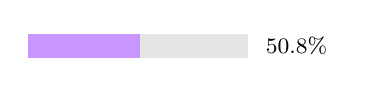
\begin{tikzpicture}
  % 背景条
  \draw[fill=gray!20,draw=none] (0,0) rectangle (2.8,0.3);
  % 进度条
  \draw[fill=lilac,draw=none] (0,0) rectangle (1.4211137162202732,0.3);
  % 百分比文本
  \node[right,font=\footnotesize] at (2.9,0.15) {50.8\%};
\end{tikzpicture}
 &
\color{lilac}\textbf{中} \\
\hline

第四章 实验验证 &
2,536 &
1,384 &


\begin{tikzpicture}
  % 背景条
  \draw[fill=gray!20,draw=none] (0,0) rectangle (2.8,0.3);
  % 进度条
  \draw[fill=lilac,draw=none] (0,0) rectangle (1.5287773247601792,0.3);
  % 百分比文本
  \node[right,font=\footnotesize] at (2.9,0.15) {54.6\%};
\end{tikzpicture}
 &
\color{lilac}\textbf{中} \\
\hline

第五章 结论 &
639 &
459 &


\begin{tikzpicture}
  % 背景条
  \draw[fill=gray!20,draw=none] (0,0) rectangle (2.8,0.3);
  % 进度条
  \draw[fill=riskred,draw=none] (0,0) rectangle (2.011360387802124,0.3);
  % 百分比文本
  \node[right,font=\footnotesize] at (2.9,0.15) {71.8\%};
\end{tikzpicture}
 &
\color{riskred}\textbf{高} \\
\hline

致 谢 &
333 &
176 &


\begin{tikzpicture}
  % 背景条
  \draw[fill=gray!20,draw=none] (0,0) rectangle (2.8,0.3);
  % 进度条
  \draw[fill=lilac,draw=none] (0,0) rectangle (1.4828629195690155,0.3);
  % 百分比文本
  \node[right,font=\footnotesize] at (2.9,0.15) {53.0\%};
\end{tikzpicture}
 &
\color{lilac}\textbf{中} \\
\hline

\end{longtable}
\end{center}

\vspace{1cm}

% 图例说明
\begin{center}
\begin{tabular}{@{}cl@{}cl@{}cl@{}cl@{}cl@{}}
\color{safegreen}$\blacksquare$ & 低风险 (<40\%) &
\color{warningyellow}$\blacksquare$ & 较低风险 (40-50\%) &
\color{lilac}$\blacksquare$ & 中等风险 (50-60\%) \\
\color{warningorange}$\blacksquare$ & 较高风险 (60-70\%) &
\color{riskred}$\blacksquare$ & 高风险 ($\ge$70\%) &
\end{tabular}
\end{center}

\end{document}

